\documentclass[openany, 11pt]{book}
\makeindex

\usepackage{amsmath}
\usepackage{amssymb}
\usepackage{booktabs}
\usepackage{csvsimple-l3}
\usepackage{bussproofs}
\usepackage{dirtytalk}
\usepackage[dvipsnames]{xcolor}
\usepackage{enumitem}
\usepackage{epigraph}
\usepackage{forest}
\usepackage{formal-grammar}
\usepackage[toc]{glossaries}
\usepackage{graphicx}
\usepackage[citecolor=blue,colorlinks=true, linkcolor=blue, urlcolor=blue]{hyperref}
\usepackage{kantlipsum}
\usepackage{makeidx}
\usepackage[margin=0.8in]{geometry}
\usepackage{mathrsfs}
\usepackage{minted}
\usepackage{multicol}
\usepackage{standalone}
\usepackage[style=authortitle]{biblatex}
\usepackage[T1]{fontenc}
\usepackage[tableaux]{prooftrees}
\usepackage{tcolorbox}
\usepackage{tikz}
\usepackage{titlesec}
\usepackage{xcolor}

\usetikzlibrary{arrows}
\usetikzlibrary{arrows.meta}
\usetikzlibrary{automata}
\usetikzlibrary{calc}
\usetikzlibrary{fit}
\usetikzlibrary{petri}
\usetikzlibrary{positioning}

\tcbuselibrary{breakable}
\tcbuselibrary{listings}
\tcbuselibrary{minted}
\tcbuselibrary{skins}
\tcbuselibrary{theorems}

\newcounter{filePrg}

% \addbibresource{biblio.bib}
\setlength{\parindent}{0pt}

\renewcommand{\emph}[1]{\textit{#1}}
\setlength{\parindent}{0pt}

\newcommand\setboxcounter[2]{\setcounter{tcb@cnt@#1}{#2}}
\setlength{\parindent}{10pt}
\newcommand{\set}[1]{\{#1\}}

\definecolor{CaribbeanBlue}{RGB}{0, 206, 209} % Define Caribbean Blue
\NewTcbTheorem[list inside=definition]{definition}
{Definition}{
	breakable,
	colback=CaribbeanBlue!05,
	colframe=CaribbeanBlue!35!black,
	fonttitle=\bfseries}{th}

\NewTcbTheorem[list inside=intuition]{intuition}{Intuition}{
	breakable,
	colback=blue!5,
	colframe=blue!35!black,
	fonttitle=\bfseries}{th}

\NewTcbTheorem{example}{Example}{
	breakable,
	colback=white,
	colframe=green!35!black,
	fonttitle=\bfseries}{th}

\NewTcbTheorem{verify}{Verify}{
	breakable,
	float,
	colback=red!5,
	colframe=red!35!black,
	fonttitle=\bfseries}{th}

\NewTcbTheorem[list inside=theorem]{theorem}{Theorem}{
	breakable,
	colback=gray!10,
	colframe=gray!35!black,
	fonttitle=\bfseries}{th}

\NewTcbTheorem[
	list inside=exercise,
	number within=section
]
{exercise}{Exercise}{
	breakable,
	colback=white,
	colframe=black,
	fonttitle=\bfseries}{th}

\newcommand{\hask}[1]{\mintinline{haskell}{#1}}

\newenvironment{alist}
{\begin{enumerate}[label={*}, leftmargin=*, itemsep=0pt, parsep=0pt]}
		{\end{enumerate}}

\newenvironment{blist}
{\begin{enumerate}[label={}, leftmargin=*, itemsep=0pt, parsep=0pt]}
		{\end{enumerate}}


\renewcommand{\thesection}{\arabic{section}}
\tcbset{enhanced jigsaw}

\newtcbinputlisting{\codeFromFile}[2]{
	listing file={#1},
	listing engine=minted,
	minted style=colorful,
	minted language=haskell,
	minted options={breaklines,linenos,numbersep=3mm},
	colback=blue!5!white,colframe=blue!75!black,listing only,
	left=5mm,enhanced,
	title={#2},
	overlay={\begin{tcbclipinterior}\fill[red!20!blue!20!white] (frame.south west)
				rectangle ([xshift=5mm]frame.north west);\end{tcbclipinterior}}
}

\newtcblisting{haskell}[1]
{
	listing engine=minted,
	minted style=colorful,
	minted language=haskell,
	minted options={breaklines,linenos,numbersep=3mm},
	colback=blue!5!white,colframe=blue!75!black,listing only,
	left=5mm,enhanced,
	title={#1},
	overlay={\begin{tcbclipinterior}\fill[red!20!blue!20!white] (frame.south west)
				rectangle ([xshift=5mm]frame.north west);\end{tcbclipinterior}}
}

\newtcblisting{shell}[1]
{
	listing engine=minted,
	minted style=colorful,
	minted language=shell,
	minted options={breaklines,linenos,numbersep=3mm},
	colback=blue!5!white,colframe=blue!75!black,listing only,
	left=5mm,enhanced,
	title={#1},
	overlay={\begin{tcbclipinterior}\fill[red!20!blue!20!white] (frame.south west)
				rectangle ([xshift=5mm]frame.north west);\end{tcbclipinterior}}
}


\begin{document}
\maketitle{}
\tableofcontents
\tcblistof[\section]{definition}{List of Definitions}
\listoffigures
\listoftables

\chapter{Type Inference}

\begin{enumerate}[label = {(\alph*)}]
	\item asdf
	\item asdf
\end{enumerate}

\begin{intuition}{Type Inference}
	The essense of type inference is walking the abstract syntax tree and
	collect constraints we must satisfy. Therefore we would reformulate the
	problem to so-called unification problem.
\end{intuition}

\begin{definition}{Type Inference}{}
	Figuring out whether an expression $e$ is well-typed, and if so, what it's
	type $T$ is $e: T$.
\end{definition}

\begin{definition}{Type Inference By Hand}{}
	We can approximate this algorithm by
	\begin{enumerate}
		\item assigning a fresh type variable to each bound name
		\item assigning a fresh type variable to the function return value
		\item solving type constraints until there is nothing more to do.
	\end{enumerate}
\end{definition}

\section{Example}
\begin{haskell}{}
	myFun w x y z = if y then w : tail x else y : z
\end{haskell}

\begin{figure}[H]
	\begin{center}
		\documentclass{standalone}
\usepackage{tikz}
\begin{document}
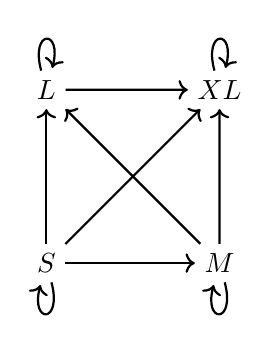
\begin{tikzpicture}[scale=1.1]
    \tikzset{arc lines/.style={thick,black, ->}}
    \node (S) at (0, 0) {$S$};
    \node (M) at (2, 0) {$M$};
    \node (L) at (0, 2) {$L$};
    \node (XL) at (2, 2) {$XL$};
    \draw [arc lines] (S) to (M);
    \draw [arc lines] (S) to (L);
    \draw [arc lines] (S) to (XL);
    \draw [arc lines] (M) to (L);
    \draw [arc lines] (M) to (XL);
    \draw [arc lines] (L) to (XL);
    \path [-stealth, thick]
        (S) edge [loop below] (S)
        (M) edge [loop below] (M)
        (L) edge [loop above] (L)
        (XL) edge [loop above] (XL)
        ;
\end{tikzpicture}
\end{document}

	\end{center}
	\caption{Toset}
\end{figure}

\section{Example}
\begin{center}
	\begin{forest}
		[\hask{=}
			[\hask{z}
				[\hask{f}]
			]
			[\hask{f}
				[\hask{(,)}
					[\hask{f}
						[\hask{3} ]
					]
					[\hask{f}
						[\hask{3} ]
					]
				]
			]
		]
	\end{forest}
\end{center}


\chapter{Functor}
\epigraph{
	There are two keys to an expert Haskell hacker’s wisdom. First understand
	the types. Next gain a deep intuition for each type class and its
	relationship to other type classes, backed up by familiarity with many
	examples.
}{Brent Yorgey}

% \printbibliography{}
% \printindex{}
\end{document}
